\chapter{Einführung}
%- Hintergrund
%- Motivation
%- Ziele
%- Aufgaben
%- Allgemeine Beschreibung des Projektes
%- Worum geht es in dieser Arbeit?
%- Wer hat die Arbeit veranlasst und wozu?
%- Wer soll von den Ergebnissen profitieren?
%- Welches Problem soll gelöst werden? Warum?
%- Unter welchen Umständen braucht man eine Verbesserung?
%- Was ist der Stand der Technik?
%- Welche noch offenen Probleme gibt es?
%- Worin unterscheidet sich mein Ansatz von den bisherigen?
%- Welche Ziele hat die Arbeit?
%- Wie will ich diese Ziele erreichen?
%- Was habe ich im Einzelnen vor?

\todo{Umformulierung?}
Die gegenwärtig stark einhergehende Digitalisierung des privaten, beruflichen und öffentlichen Lebens verändert die Art wie Unternehmen untereinander konkurrieren, Werte schaffen und mit ihren Geschäftspartnern und Kunden interagieren \cite[S. 1]{oswald_digitale_2018}.

Die sogenannte Digitale Transformation wird ein zunehmend wichtig werdender Veränderungsprozess, um die gegenwärtigen Potenziale neuer Innovationen wie Big Data, künstliche Intelligenz oder Cloud Computing konsequent auszunutzen und stetig Wettbewerbsvorteile zu generieren \cite<vgl.>[S. 2]{oswald_digitale_2018}. Klassische Führungskonzepte greifen nicht mehr, Stichworte wie Flexibilität, Schnelligkeit, Dynamik und Kundenorientierung sind essentielle Voraussetzungen. 

Das Aufbrechen alteingesessener Strukturen bis hin zur Transformation zu einem digitalen Unternehmen bringt jedoch hohe Probleme mit sich. Bei einer erfolgreichen Umsetzung des Veränderungsprozesses spielen eine große Reihe von Einflüssen mit ein. Oft bremsen gerade alte Strukturen den Erfolg der Veränderungen, was gerade bei der Forderung nach Flexibilität und Dynamik ein großes Problem darstellt
\cite<vgl.>[S. 196]{appelfeller_digitale_2018}


Sogenannte agile Methoden können helfen, Probleme des klassischen Change Managements in der Digitalen Transformation zu bearbeiten. Praktiken wie z.B. Design-Thinking oder DevOps haben sich bereits als Projektmanagement-Instrumente bewährt \cite<vgl.>[S. 7]{deeken_agiles_2018}. Interessant ist jedoch auch die Herangehensweise, sie im größeren Umfeld einer Organisationskultur einzusetzen, um mithilfe der Bildung einer Agilen Kultur den Transformationsprozess zu optimieren \cite<vgl. >[S. 140]{hofert_agiler_2016}.

Im Folgenden soll auf das genaue Forschungsschwerpunkt der vorliegenden Arbeit eingegangen werden. Es wird eine Einführung über Problematiken innerhalb der Digitalen Transformation gegeben und die exakte Zielstellung der Arbeit aufgeführt. Außerdem wird nachfolgend der genaue Aufbau der Arbeit geklärt und mithilfe welcher Methodik die aufgeführten Fragestellungen beantwortet werden sollen.

\section{Problemstellung}

''Die Diskussion rund um digitale Transformation ist geprägt von Hypes und dringenden Warnungen, die zum Handeln anregen sollen.'' \cite[S. 12]{berghaus_2016}. Innerhalb der Digitalisierung kommt es zu einem zunehmenden Druck um die Aufrechterhaltung eines konkurrenzfähigen Geschäftsmodells. Das Aufkommen immer neuer Innovationen in verschiedenen Technologien bildet zudem eine Gefährdung durch neue Möglichkeiten von Markteintritten, bis hin zur Zerschlagung altbewährter Geschäftsmodelle, sogenannte Digitalen Disruptionen \cite<vgl.>{urbach_digitalization_2018}.

Diese Gefährdungen treiben Großunternehmen dazu, gegenwärtige Strukturen zu überdenken und Veränderungen einzuleiten. \todo{Zitat finden!} Vornehmlich die Digitalisierung des Geschäftsmodells, aber auch der gesamten Unternehmensstruktur samt - kultur sind wichtige Themen in den Führungsebenen großer, internationaler Unternehmen \cite<vgl.>[S. 18]{buhse_transformationswerk_2016}. Das Bestreben nach Veränderungen hin zu einem digitalen Unternehmen ist also erkennbar in den Köpfen von Management und Führung. Trotzdem lassen Studien wie von \citeA{buhse_transformationswerk_2016} erkennen, dass solch ein großangelegter Veränderungsprozess wie die Digitale Transformation ebenso große Problemfelder mit sich bringen kann. Oft mangelt es schon an erfolgreicher Kommunikation innerhalb des Unternehmen, beispielsweise hervorgerufen durch ''existente Vernetzungslücken und Defizite in der internen Kommunikation'' \cite[S. 18]{buhse_transformationswerk_2016}.

Zur Bekämpfung klassischer Probleme in großen Veränderungsprozessen bedarf es oft externer Hilfe. Promotoren oder Inkubatoren können helfen, Problemfelder im Transformationsprozess anzugehen \todo{Zitat Kaune Buch?}. \citeauthor{zillmann_status_2017} geht in seiner Studie sogar soweit, dass ''$\lbrack$o$\rbrack$hne externe Beratungs- und IT-Dienstleister $\lbrack$...$\rbrack$ all diese Herausforderungen nicht zu bewältigen'' (S. 16) wären. Interne Treiber können aber ebenfalls dazu beitragen, solche Problemfelder anzugehen. Oft fehlt es allein schon an kulturellen Veränderungen innerhalb des Unternehmens \cite<vgl.>{hofert_agiler_2016} \todo{Seite?}. Ein sogenanntes ''Agiles Mindset'' kann helfen, einen  solchen ''Kulturwandel'' einzuleiten \cite<vgl.>{hofert_agile_2018}.

Eine wesentliche Fragestellung der vorliegenden Arbeit soll es sein, eine Reihe solcher Problemfeldern zu identifizieren, die eine angestrebte Digitale Transformation gefährden. Daraus resultierend soll untersucht werden, inwieweit der Einsatz sogenannter Agiler Praktiken diese lösen können.

\section{Forschungsfragen und Zielstellung}

% - Darstellung der Forschungsfragen (siehe Exposé!)

\todots

\section{Aufbau der Arbeit}

% - modularer Aufbau, zu Erstellen: Grafik, woraus ersichtlich wird, wie die einzelnen Kapitel zusammenhängen
\begin{figure}[H]
	\centering
	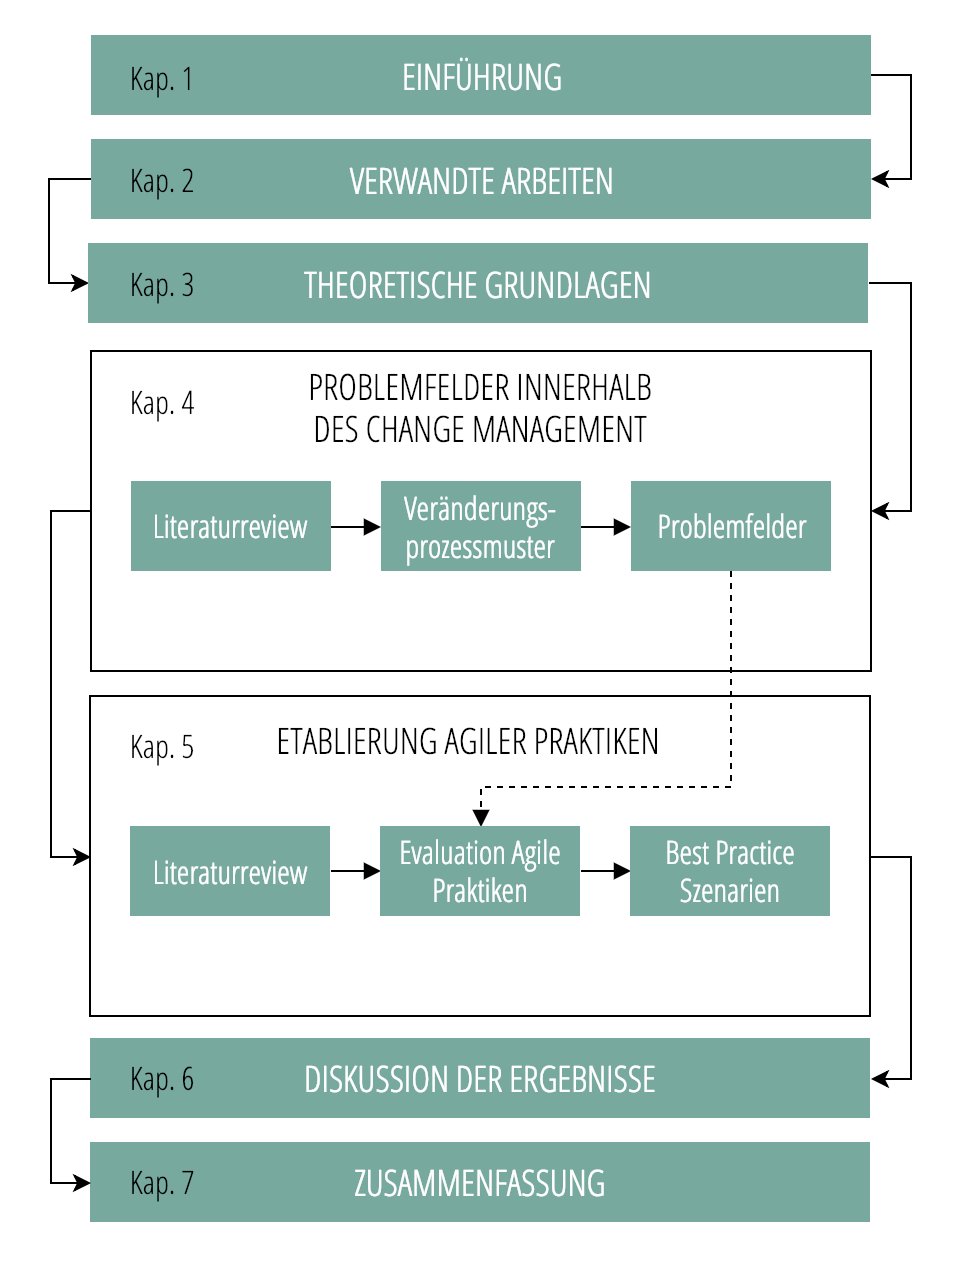
\includegraphics[width=0.5\linewidth]{pics/aufbau}
	\caption{Aufbauschema der Arbeit}
	\label{fig:aufbau}
\end{figure}



\todots

\section{Methodisches Vorgehen}

% - allgemeines Vorgehen, mit Verweis auf die methodischen Unterkapitel der einzelnen Abschnitte. Systematischer Literaturreview + Metastudie als spezielle Form, Evaluation am Ende der zweiten Metastudie

\todots
